\chapter{Majorization theory} \label{chap:majorization}

Notations for majorization theory mostly follow Ref. \cite{marshall_inequalities_2011}, except for the reordering convention $p^\downarrow$ (cf. section \ref{sec:cumulative}) and notations for the majorization lattice which come from Ref. \cite{cicalese_supermodularity_2002}.



\section{The majorization relation} \label{sec:majorization}

The theory of majorization gives a framework for what it means for a probability distribution (or vectors) to be more disordered, more random, than another one. A rigorous notion of disorder such as the one that majorization suggests is interesting because it is linkable to other objects that attempt to quantify randomness in information theory, and most notably Shannon entropy. In order to see that this is the case, we first need to rigorously define the majorization relation.



\subsection{Definition using cumulative sums} \label{sec:cumulative}

This section is based on Ref. \cite[pp. 4--10]{marshall_inequalities_2011}. Let $p$ be a probability vector, \textit{i.e.} a vector such that $p_i \geq 0$ and $\sum_{i}^{d} p_i = 1$ for a vector of dimension $d$. Let $p^\downarrow$ be the non-increasing reordering of $p$, meaning that the entries of $p^\downarrow$ are the same as those of $p$, but sorted such that $p^\downarrow_1 \geq p^\downarrow_2 \geq ... \geq p^\downarrow_d$. We will always be considering reordered vectors in this master thesis, and we will therefore denote the set of $d$-dimensional probability vectors sorted in non-increasing order $\mathcal{P}^d$. Formally, $\mathcal{P}^d = \{p \in \mathbb{R}^d | \sum_{i}^{d} p_i = 1, p_i \geq p_{i+1}\}$.

\begin{definition}[Cumulative sum] % ressemble beaucoup a ce que Serge a ecrit dans son memoire, a reformuler
    Let $p$ be a vector in $\mathcal{P}^d$. The $k^{\text{th}}$ non-increasing\footnote{We could also have defined $\mathcal{P}^d$ to be non-decreasing vectors and use non-decreasing cumulative sums $S^\uparrow_i (p)$ instead. We would get an equivalent description of majorization, the only effect being reversed inequalities in (\ref{eq:majorization}).} cumulative sum of $p$ is the sum of the $j$ biggest components of $p$, which can be written as
    \begin{equation}
        S^\downarrow_k (p) \coloneqq \sum_{i = 1}^{k} p^\downarrow_i,
    \end{equation}
    where $p^\downarrow_i$ is the $i^{\text{th}}$ largest entry of $p$. 
\end{definition}

\begin{definition}[Majorization relation] \label{def:majorization}
    Let $p, q \in \mathbb{R}^d$ be two vectors of dimension $d$. We say that $p$ is majorized by $q$, written $p \prec q$, if and only if
    \begin{equation} \label{eq:majorization}
        \begin{system}
            S^\downarrow_k (q) \geq S^\downarrow_k (p) \quad \forall k = 1,...,d - 1, \\
            S^\downarrow_d (q) = S^\downarrow_d (p).
        \end{system}
    \end{equation}
If the dimensions of the vectors do not match, one can always append zeroes to the one of lower dimension and apply the definition on the enlarged vector.
\end{definition}

\begin{remark}
    If $p$ and $q$ are probability vectors, then the last equality is automatically verified because $S^\downarrow_d (p) = S^\downarrow_d (q) = 1$.
\end{remark}

This definition encapsulates the idea of disorder: if $p \prec q$, then the largest probability of $q$ ($q_1^\downarrow)$ is larger than the largest probability of $p$ ($p_1^\downarrow$), and the rest of the distribution in $q$ is lowered for the sum of probabilities to give $1$, whereas $p$ has a distribution that is more spread out. As an example, consider $q = (0.9, 0.1)$ and $p = (0.6, 0.4)$, and applying Definition \ref{def:majorization} we see that $p \prec q$. This feels fairly intuitive : $q$ is not as uncertain as $p$, because a process described by probability distribution $q$ sees one of the 2 events happen most of the time, whereas the outcome of a process with probability distribution $p$ is almost equally likely to be one or the other. It is clear from this example that the \textit{majorizer} is more ordered than the \textit{majorized}.

\begin{remark}
    For any $p \in \mathcal{P}^d$, we have
    \begin{equation} \label{eq:top_bottom}
        \left(\frac{1}{d}, ..., \frac{1}{d}\right) \prec p \prec (1, 0, ..., 0)
    \end{equation}
    which is fairly intuitive, considering that $(\frac{1}{d}, ..., \frac{1}{d})$ is the most uncertain distribution and $(1, 0, ..., 0)$ is the most certain distribution. % ca ressemble beaucoup a ce que Serge a ecrit dans son memoire, a reformuler
\end{remark}

The majorization relation creates a partial order on $\mathcal{P}^d$, meaning that the ordering is both reflexive and transitive on the set, and that\footnote{This is not the case if we choose the subset of $\mathbb{R}^d$  of vectors with non-negative entries, where having both $p \succ q$ and $p \prec q$ only means that $p$ and $q$ are the same up to a reordering. On non-ordered vectors, the majorization relation therefore only generates a preorder instead of a proper partial order.} $p \prec q$ and $p \succ q \implies p = q$ for any $p, q \in \mathcal{P}^d$. When either $p \prec q$ or $p \succ q$ is verified, we will say that $p$ and $q$ are \textit{comparable} (written $p \sim q$). However, there also exist cases where both $p \nprec q$ and $p \nsucc q$ are true, and we will then say that $p$ and $q$ are \textit{incomparable} (written $p \nsim q$). For example, $(0.5, 0.25, 0.25) \nsim (0.4, 0.4, 0.2)$.

\begin{remark}
    Two vectors of dimension 2 are always comparable. Incomparability is only possible from dimension 3 and above.
\end{remark}



\subsection{Definition using bistochastic matrices} \label{sec:bistochastic}

This section is based on Ref. \cite[pp. 29--33]{marshall_inequalities_2011}. A second equivalent definition for majorization can be reached by a different intuition involving bistochastic matrices. The idea is the following: if the probability vector $q$ can be obtained by randomly mixing the components of $p$ together, then $p$ is more ordered than $q$. It turns out that this simple idea is equivalent to the definition using cumulative sums. Let us express this rigorously.

\begin{definition}[Bistochastic matrix]
    A bistochastic matrix $D$ is a matrix in $\mathbb{R}^{d \times d}$ such that
    \begin{equation}
        \begin{system}
            D_{i,j} \geq 0 \quad \forall i,j = 1, ..., d \\
            \sum_{i = 1}^{d} D_{i, j} = 1 \quad \forall j = 1, ..., d \\
            \sum_{j = 1}^{d} D_{i, j} = 1 \quad \forall i = 1, ..., d
        \end{system}
    \end{equation}
\end{definition}

A bistochastic matrix (also called doubly stochastic matrix) is basically a matrix with nonnegative entries such that the columns and rows each sum to one. The following theorem formalizes the way that bistochastic matrices mix entries of vectors together.

\begin{theorem}[Birkhoff's theorem] \label{th:birkhoff}
    If $D$ is a $d$-dimensional bistochastic matrix, then there exists a probability distribution $\{p_j\}$ and a set of $d$-dimensional permutation matrices $P_j$ such that
    \begin{equation} \label{eq:birkhoff}
        D = \sum_{j} p_j P_j
    \end{equation}
\end{theorem}

From this theorem, we can see that the effect of a bistochastic matrix on a vector is essentially to perform a convex mixture of the vector's entries, producing a vector that is more smoothed out, and thus more disordered.

\begin{theorem}[Hardy, Littlewood and Pólya] \label{th:bistochastic_majorization}
    Let $p, q \in \mathcal{P}^d$. Then, $p \prec q$ if and only if there exists a $d$-dimensional bistochastic matrix $D$ such that
    \begin{equation} \label{eq:bistochastic_majorization}
        p = Dq.
    \end{equation}
\end{theorem}

One can take theorem \ref{th:bistochastic_majorization} as a definition of the majorization relation, as the notion of a vector being more disordered is perhaps clearer in the bistochastic matrix picture. Then, the nature of the convex combination % Serge: expliquer ce que c'est
of entries would have given us the set of inequalities (\ref{eq:majorization}). Let's take the same example as earlier, $p = (0.6, 0.4)$ and $q = (0.9, 0.1)$. Then we can find that $D = \Big(\begin{smallmatrix}
                                                                                                    5/8 & 3/8 \\
                                                                                                    3/8 & 5/8
                                                                                                \end{smallmatrix}\Big)$
gives us $p = Dq$, and therefore $p \prec q$.

Whichever picture one prefers intuitively, the fact that there is a full equivalence between the two is quite powerful when working on proofs, as sometimes one picture is easier to work with than the other depending on the context.

\begin{remark}
    The bistochastic matrix $\begin{pmatrix} \frac{1}{d} & \dots & \frac{1}{d} \\
                                                      \vdots & & \vdots \\
                                                      \frac{1}{d} & \dots & \frac{1}{d}
                             \end{pmatrix}$ 
    produces the probability vector $(\frac{1}{d}, \dots, \frac{1}{d})$ regardless of the probability vector on which it is applied, hence $(\frac{1}{d}, \dots, \frac{1}{d})$ is majorized by every probability vector in $\mathcal{P}^d$.
\end{remark}



\subsection{Visualization using Lorenz curves}

This section is based on Ref. \cite[pp. 5--6]{marshall_inequalities_2011}. Lorenz curves were first introduced in 1905 by economist Max Lorenz as a way to represent income inequality. By plotting the cumulative sums of two distributions, we can say that if one curve is above the other at all times, then it is more unequal (more disordered) than the second. By normalizing the distributions for total income, this graphical tool could then be used to quickly compare income inequality between different regions or countries.

More formally, the Lorenz curve of a vector $p \in \mathbb{R}^d$ is obtained by linear interpolation between the points of the set $\{(i, S^\downarrow_i(p)) | i \in \mathbb{N}, i \leq d\}$.
We will be using the convention that $S^\downarrow_0 (v) = 0$ for any vector $v$. A couple of examples are given in figures \ref{fig:lorenz_comparable_example} and \ref{fig:lorenz_incomparable_example}.

\begin{figure}[h!]
    \centering
    \begin{minipage}{.48\textwidth}
        \centering
        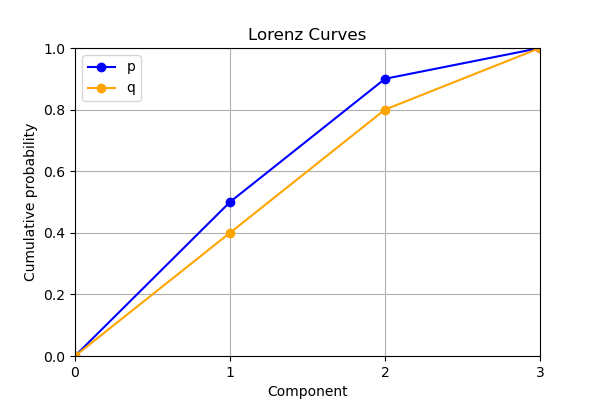
\includegraphics[scale=0.45]{images/lorenz_comp.png}
        \caption{Lorenz curves for comparable vectors $p = (0.5, 0.4, 0.1)$, $q = (0.4, 0.4, 0.2)$.}
        \label{fig:lorenz_comparable_example}
    \end{minipage}
    \hfill
    \begin{minipage}{0.48\textwidth}
        \centering
        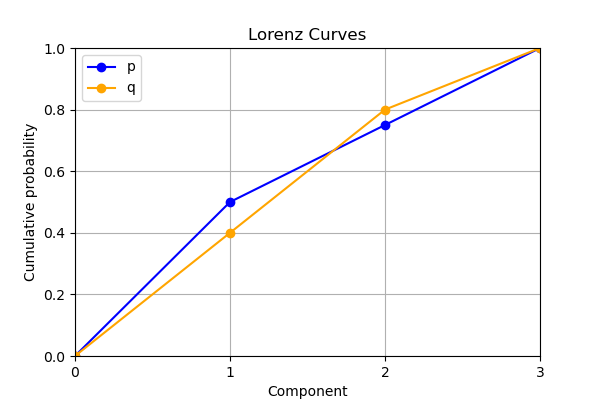
\includegraphics[scale=0.45]{images/lorenz_incomp.png}
        \caption{Lorenz curves for incomparable vectors $p = (0.5, 0.25, 0.25)$, $q = (0.4, 0.4, 0.2)$.}
        \label{fig:lorenz_incomparable_example}
    \end{minipage}
\end{figure}

At integer abscissa $i$, we see the values of $S_i^\downarrow (v)$ for each vector $v$. At each point, we can thus compare the value of the cumulative sums of each vector, which is precisely the same as an inequality of the majorization relation \ref{eq:majorization}. From these figures, we quite quickly get the intuition that if one vector majorizes another (i.e. they are comparable), then all of the inequalities must be satisfied and the majorizer's curve must be above the majorized's curve at all points. If the two vectors are incomparable, then at least one inequality must fail, and so there must be a reversal in the largest cumulative sum, and the Lorenz curves must cross at least once.

\subsection{Weak majorization}

This section is based on \cite[pp. 10--15]{marshall_inequalities_2011}. It is sometimes useful to relax a bit the conditions on the majorization relation, in order to compare vectors that do not have the same sum. Two complementary notions can be defined, \textit{submajorization} and \textit{supermajorization}.

\begin{definition}[Submajorization] \label{def:submajorization}
    Let $p, q \in \mathbb{R}^d$ be two vectors of dimension $d$. We say that $p$ is submajorized by $q$, written $p \prec_w q$, if and only if
    \begin{equation} \label{eq:submajorization}
            S^\downarrow_k (q) \geq S^\downarrow_k (p) \quad \forall k = 1,...,d.
    \end{equation}
If the dimensions of the vectors do not match, one can always append zeroes to the one of lower dimension and apply the definition on the enlarged vector.
\end{definition}

\begin{definition}[Supermajorization] \label{def:supermajorization}
    Let $p, q \in \mathbb{R}^d$ be two vectors of dimension $d$. We say that $p$ is supermajorized by $q$, written $p \prec^w q$, if and only if
    \begin{equation} \label{eq:supermajorization}
            S^\uparrow_k (q) \leq S^\uparrow_k (p) \quad \forall k = 1,...,d,
    \end{equation}
where $S^\uparrow_k(p)$ and $S^\uparrow_k (q)$ denote the $k^\text{th}$ non-decreasing cumulative sums\footnote{Notice that using the reverse ordering means that the first components of $p^\uparrow$ are the smallest components of $p$, and so the smallest components of $p$ should be greater than those of $q$ in order to be more uncertain. This is why the inequality in equation (\ref{eq:supermajorization}) is reversed.} of $p$ and $q$. If the dimensions of the vectors do not match, one can always append zeroes to the one of lower dimension and apply the definition on the enlarged vector.
\end{definition}

Essentially, these definitions are the same as majorization, but they remove the condition that $S_d(p) = S_d(q)$. This allows to compare objects that do not have the same 1-norm.

FAIRE UNE PAIRE DE COURBES DE LORENZ





\section{Schur-convex and Schur-concave functions}

\subsection{Definition}

This section is based on Ref. \cite[pp. 79--92]{marshall_inequalities_2011}. Some functions preserve the ordering defined by the majorization relation and are therefore interesting to study because a majorization relation directly implies an inequality on these functions. The following few definitions will be useful.

\begin{definition}[Convex function]
    A function $f \in C(\mathcal{I} \to \mathbb{R})$ is convex on an interval $\mathcal{I}$ iff for all $x_1, x_2 \in \mathcal{I}$
    \begin{equation}
        f(\alpha x_1 + (1-\alpha) x_2) \leq \alpha f(x_1) + (1-\alpha) f(x_2) \quad \forall \alpha \in [0, 1].
    \end{equation}
\end{definition}

\begin{definition}[Schur-convex function]
    A function $f \in C(\mathbb{R}^d \to \mathbb{R})$ is Schur-convex iff for all $p, q \in \mathcal{P}^d$
    \begin{equation}
        p \prec q \implies f(p) \leq f(q).
    \end{equation}
\end{definition}

Conversely, a function $f$ is (Schur-)concave if $-f$ is (Schur-)convex. Additional properties linking convex and concave functions to majorization exist.

\begin{lemma}[Karamata's inequality] \label{lem:karamata}
    If $f \in C(\mathcal{I} \to \mathbb{R})$ is convex on $\mathcal{I}$, and if $p \prec q$, then
    \begin{equation}
        \sum_{i=1}^{d} f(p_i) \leq \sum_{i=1}^{d} f(q_i).
    \end{equation}
    This can be restated as saying that the function $\sum_i f$ is Schur-convex.
\end{lemma}

Essentially, this inequality states that if $b = Da$ with $D$ a bistochastic matrix, then $a$ has entries that are more spread out (think of the certain vector), whereas $b$ has entries closer to the middle of the interval (think of the uniform vector), and so, by definition of a convex (resp. concave) function, on average $f(b_i)$ is less (resp. more) than $f(a_i)$.



\subsection{Shannon entropy} \label{sec:schur_shannon}

This section is based on Refs. \cite[p. 101]{marshall_inequalities_2011} and \cite[p. 88]{cover_elements_2006}. % pas sur que citer un exercice soit hyper acceptable mdr
The Shannon entropy function $H(p) \coloneqq - \sum_{i = 1}^{d} p_i \log p_i$ is a foundational quantity in classical information theory (cf. section \ref{sec:classical_information}). $H(p)$ essentially captures the uncertainty content of a random process distributed over a probability distribution $p$. We therefore expect it to be linked to majorization theory which gives a partial order on the uncertainty of different probability distributions. The following lemma establishes this link through Schur-concavity.

\begin{lemma}[Schur-concavity of the Shannon entropy]
    For any $p, q \in \mathcal{P}^d$,
    \begin{equation}
        p \prec q \implies  H(p) \geq H(q).
    \end{equation}
\end{lemma}

This property of Shannon entropy is fairly intuitive: the Shannon entropy captures the uncertainty content of a probability distribution, and $p \prec q$ means that $q$ is unequivocally\footnote{As opposed to incomparable distributions being more ordered than the other each in their own way.} more ordered (so more certain) than $p$, so we would expect Schur-concavity to hold. However a majorization relation is stronger than an entropic inequality, and so we should study majorization relations alongside Shannon entropy to gain a better understanding of information theory.
% Il existe une version plus forte de ce lemme, p \succ q implique H(q) - H(p) \geq D(p^\downarrow \parallel q^\downarrow) dans \cite{ho_interplay_2010}

\subsection{Rényi entropies}





\section{Majorization lattice} \label{sec:majorization_lattice}

\subsection{Lattice structures}

This section is based on \cite{cicalese_supermodularity_2002}. The majorization relation creates a proper partial ordering on the set of \textit{ordered} probability vectors $\mathcal{P}^d$. With the ordering induced by the majorization relation, the set of ordered vectors $\{z | z_1 \geq z_2 \geq ... \geq z_d\}$ becomes a lattice.

\begin{definition}[Lattice] \label{def:lattice} % copie colle de l'article de Cicalese and Vaccaro, c'est ok ou pas ?
    A lattice is a quadruple $\langle \mathcal{L}, \sqsubseteq, \wedge, \vee \rangle$ where $\mathcal{L}$ is a set, $\sqsubseteq$ is a partial ordering $\mathcal{L}$, and for all $a, b \in \mathcal{L}$ there is a unique greatest lower bound (glb) $a \wedge b$ and a unique least upper bound (lub) $a \vee b$. That is, $a \wedge b$ precedes ($\sqsubseteq$) both $a$ and $b$ and $a \vee b$ succedes ($\sqsupseteq$) both $a$ and $b$, and for any $c$ that precedes both $a$ and $b$, and for any $d$ that succedes both $a$ and $b$, we have
    \begin{equation}
        c \sqsubseteq a \wedge b \quad \text{and} \quad a \vee b \sqsubseteq d.
    \end{equation}
\end{definition}

A simple example of a lattice is the set $\mathbb{N}$ of natural numbers ordered by the relation “divides”. Then for $a, b \in \mathbb{N}$ the lub is the least common multiple of $(a, b)$ and the glb is the greatest common divisor of $(a, b)$. % example from Dominich, 2008, Elements of Lattice Theory

It was shown that the set $\mathcal{P}^d$ endowed with the partial ordering $\prec$ is a lattice. As the lattice is a central part of this master thesis, we will go through the main ideas behind the proof, which hinges on defining the correct greatest lower bound (glb) $p \wedge q$, which is called the \textit{meet} of $p$ and $q$, and the correct least upper bound (lub) $p \vee q$, which is called the \textit{join}.

Let us first go through what it means for a vector to be the glb, the meet, of two vectors $p, q \in \mathcal{P}^d$. Intuitively, the glb of $p$ and $q$ in terms of majorization is the least disordered vector that is majorized by both $p$ and $q$. While this may not seem very interesting at a first glance, recall that two vectors may be incomparable, meaning that both $p \nprec q$ and $p \nsucc q$ are true. Even if they are incomparable, the subset of vectors that are majorized by both $p$ and $q$ is nonempty\footnote{It is guaranteed to at least contain the uniform distribution $(\frac{1}{d}, ..., \frac{1}{d})$ since it is majorized by every other distribution.} and has a supremum, $p \wedge q$, \textit{which majorizes every other vector in the subset}. Note that an equivalent definition of a lattice is to require that every partially ordered subset has a supremum and infimum \cite[p. 19]{marshall_inequalities_2011}. Since the two definitions are equivalent, we can consider this to be a property of the lattice, guaranteeing the existence of the supremum $p \wedge q$.

In similar fashion, the lub, the join, of two vectors $p, q \in \mathcal{P}^d$ is the least ordered vector that majorizes both $p$ and $q$. The subset of vectors that majorize both $p$ and $q$ is nonempty\footnote{It is guaranteed to at least contain the certain distribution $(1, 0, ..., 0)$ since it majorizes every other distribution.} and has an infimum, $p \vee q$, \textit{which is majorized by every other vector in the subset}. Moreover, the same property as before guarantees the existence of the infimum.

\begin{corollary} \label{cor:comp_meet_join}
    If two vectors are comparable, say $p \prec q$ (the $p \succ q$ case being symmetric), then the question becomes trivial as the least ordered vector that majorizes both $p$ and $q$ is $q$ and the least disordered vector that is majorized by both $p$ and $q$ is $p$, i.e. $p \wedge q = p$ and $p \vee q = q$.
\end{corollary}



\subsection{Majorization cones and geometric intuition} \label{sec:majorization_cones}

Before going further with the proof, let us first give a 2D visual representation of the lattice, which is very helpful in building intuition for using the lattice, first proposed in the field of thermomajorization \cite{korzekwa_structure_2017}. More accurate representations exist but are much more complicated, living in the canonical Weyl chamber of a $\Delta_{d-1}$ simplex \cite{junior_geometric_2022}. Nevertheless, the simple 2D depiction is very useful to think about, even if one has to be careful not to draw hasty conclusions from it.

\begin{definition}[Majorization cones] \label{def:majorization_cones}
    The set of states that majorize $p$ is called the \textit{future cone}\footnote{Our naming conventions and notations are for the most part entirely opposite to the thermomajorization conventions for reasons that will be made clear in section \ref{sec:nielsen}. Most notably, our future cone corresponds to their past cone and vice versa.}  $\mathcal{T}_+ (p)$. The set of states that are majorized by $p$ is called the \textit{past cone} $\mathcal{T}_- (p)$. The set of states that are neither in the past nor the future cone of $p$ is called the \textit{incomparable region} $\mathcal{T}_\emptyset (p)$.
\end{definition}

Figure \ref{fig:maj_cones_example} shows an example of the 2D representation of a vector $p \in \mathcal{P}^d$ in the lattice, along with some definitions we introduce now, and figure \ref{fig:meet_join_example} shows the intersections of the majorization cones of two vectors $p, q \in \mathcal{P}^d$ and their meet and join.

\begin{figure}[h!]
    \centering
    \begin{tikzpicture}[scale=0.9]
        % draw cone of p
        \coordinate (A) at (-2,3);
        \coordinate (B) at (2, -3);
        \draw [name path=A--B] (A) -- (B);
        \coordinate (C) at (-2,-3);
        \coordinate (D) at (2,3);
        \draw [name path=C--D] (C) -- (D);
        \path [name intersections={of=A--B and C--D,by=E}];
        \node [fill=black,inner sep=1pt,label=0:$p$] at (E) {};
        % fill draw the future cone of p + notation
        \fill[fill=red, opacity=0.2] (C) -- (E) -- (B) -- cycle;
        \node [inner sep=0pt, label=-90:$\mathcal{T}_+ (p)$] at (0, -2) {};
        % fill draw the past cone of p + notation
        \fill[fill=blue, opacity=0.2] (A) -- (E) -- (D) -- cycle;
        \node [inner sep=0pt, label=90:$\mathcal{T}_- (p)$] at (0, 2) {};
        % fill draw the incomparable region of p mais pas hyper clair
        %\filldraw[draw=black, fill=gray, opacity=0.2] (A) -- (E) -- (C) -- cycle;
        %\filldraw[draw=black, fill=gray, opacity=0.2] (D) -- (E) -- (B) -- cycle;
        \node [inner sep=0pt, label=0:$\mathcal{T}_\emptyset (p)$] at (1.5, 0) {};
        % create the entropy arrow
        \coordinate (F) at (-3, -2);
        \coordinate (G) at (-3, 2);
        \draw[->] (F) -- (G);
        \node [inner sep=0pt, label=0:Entropy] at (-3, 0) {};
        
    \end{tikzpicture}
    \caption{Depiction of the majorization cones of a nondescript vector $p \in \mathcal{P}^d$.}
    \label{fig:maj_cones_example}
\end{figure}

\begin{figure}[h!]
    \centering
    \begin{tikzpicture}[scale=0.9]
        % draw cone of p
        \coordinate (A) at (-2,3);
        \coordinate (B) at (2, -3);
        \draw [name path=A--B] (A) -- (B);
        \coordinate (C) at (-2,-3);
        \coordinate (D) at (2,3);
        \draw [name path=C--D] (C) -- (D);
        \path [name intersections={of=A--B and C--D,by=E}];
        \node [fill=black,inner sep=1pt,label=0:$p$] at (E) {};
        % draw cone of q
        \coordinate (F) at (-0.666,3);
        \coordinate (G) at (3.333, -3);
        \draw [name path=F--G] (F) -- (G);
        \coordinate (H) at (0.666,-3);
        \coordinate (I) at (4.666,3);
        \draw [name path=H--I] (H) -- (I);
        \path [name intersections={of=F--G and H--I,by=J}];
        \node [fill=black,inner sep=1pt,label=0:$q$] at (J) {};
        %intersections of the 2 cones
        \path [name intersections={of=F--G and C--D,by=K}];
        \path [name intersections={of=H--I and A--B,by=L}];
        \node [fill=black,inner sep=1pt,label=0:$p \wedge q$] at (K) {};
        \node [fill=black,inner sep=1pt,label=0:$p \vee q$] at (L) {};
        %fill the two cones
        \fill[fill=blue, opacity=0.2] (F) -- (K) -- (D) -- cycle;
        \node [inner sep=0pt] at ($ (F) !.3333! (K) !.3333! (D) $) {$\mathcal{T}_- (p \wedge q)$};
        \fill[fill=red, opacity=0.2] (H) -- (L) -- (B) -- cycle;
        \node [inner sep=5pt, label=-90:$\mathcal{T}_+ (p \vee q)$] at ($ (H) !.3333! (L) !.3333! (B) $) {};
        
    \end{tikzpicture}
    \caption{Depiction of the intersection of the majorization cones of incomparable vectors $p, q \in \mathcal{P}^d$. Note that by definition of the meet and join, $\mathcal{T}_+ (p) \cap \mathcal{T}_+ (q) = \mathcal{T}_+ (p \vee q)$ and $\mathcal{T}_- (p) \cap \mathcal{T}_- (q) = \mathcal{T}_- (p \wedge q)$.}
    \label{fig:meet_join_example}
\end{figure}

In classical and quantum information, the lattice is usually drawn with more disordered vectors at the top and more ordered vectors at the bottom because the entropy of a state is considered a resource (cf. section \ref{sec:QRT}). This means that the uniform distribution sits at the very top of the diagram, and the certain distribution at the very bottom. One should therefore be careful, because the majorization relation runs from top to bottom, which is the opposite of what one would picture at first (a greatest lower bound looks like a least upper bound and vice-versa). While this is inconvenient for this chapter, this convention will make more sense later down the road.



\subsection{Constructing the meet} \label{sec:meet}

In order to show that the quadruple $\langle \mathcal{P}^d, \prec, \wedge, \vee \rangle$ is indeed a lattice, we need to find an appropriate definition for the glb $p \wedge q$ and lub $p \vee q$ of two arbitrary elements $p$ and $q$ in $\mathcal{P}^d$. Let us start with the meet $p \wedge q$. Thinking in terms of Lorenz curves is actually very helpful here and can lead us very intuitively to the correct algorithm for constructing the meet. Let us choose the example $p = (0.6, 0.2, 0.2)$ and $q = (0.45, 0.45, 0.1)$, both in $\mathcal{P}^3$ (below dimension 3 all vectors are comparable and the lattice is trivial). Intuitively, the most ordered state that is majorized by both $p$ and $q$ should have a Lorenz curve that hugs the curves of $p$ and $q$ from below, let us write it $\alpha(p, q)$. Figure \ref{fig:meet_attempt} shows their Lorenz curves.

\begin{figure}[h!]
    \centering
    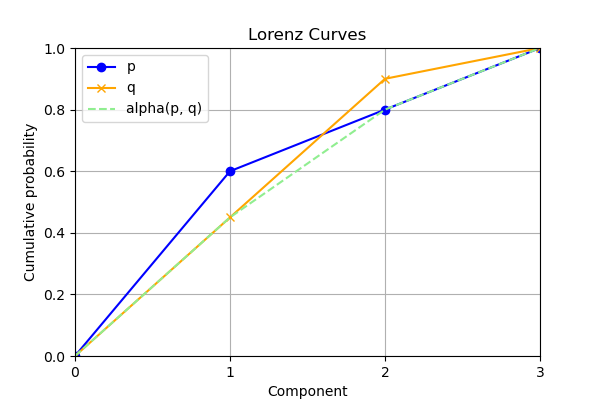
\includegraphics[scale=0.6]{images/meet_intuition.png}
    \caption{Representation of the $p = (0.6, 0.2, 0.2)$ and $q = (0.45, 0.45, 0.1)$ example, along with the proposed $\alpha(p, q)$ glb vector.} \label{fig:meet_attempt}
\end{figure}

\noindent More formally, we can define the vector $\alpha(p, q) = (a_1, \dots , a_d)$ as

\begin{align}
    a_i &= \min \Big\{ \sum_{j=1}^{i} p_j , \sum_{j=1}^{i} q_j \Big\} - \sum_{j=1}^{i-1} a_j \label{eq:alpha_bis} \\
    &= \min \Big\{ \sum_{j=1}^{i} p_j , \sum_{j=1}^{i} q_j \Big\} - \min \Big\{ \sum_{j=1}^{i-1} p_j , \sum_{j=1}^{i-1} q_j \Big\}. \label{eq:alpha}
\end{align}

\begin{lemma}[Cicalese and Vaccaro, 2002 \cite{cicalese_supermodularity_2002}] \label{lem:meet}
    For all $p, q \in \mathcal{P}^d$ we have $\alpha(p, q) = p \wedge q$.
\end{lemma}



\subsection{Constructing the join} \label{sec:join}

We can proceed in a similar way for the join of two vectors $p \vee q$, and thinking in terms of Lorenz curves will once again give us the right idea to move forward. As a first attempt, let us take $p = (0.6, 0.2, 0.2)$ and $q = (0.45, 0.45, 0.1)$ again, both in $\mathcal{P}^3$. This time, the least ordered vector that still majorizes both $p$ and $q$ should have a Lorenz curve that hugs their curves from above, let us write it $\beta(p, q)$. Figure \ref{fig:join_naive_attempt} shows their Lorenz curves.

\begin{figure}[h!] 
    \centering
    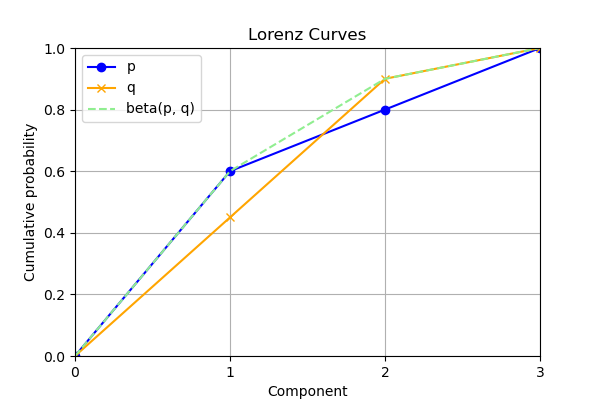
\includegraphics[scale=0.6]{images/join_naive_attempt.png}
    \caption{Representation of the $p = (0.6, 0.2, 0.2)$ and $q = (0.45, 0.45, 0.1)$ example, along with the prototype $\beta(p, q)$ lub vector.} \label{fig:join_naive_attempt}
\end{figure}

\noindent More formally, we can define the vector $\beta(p, q) = (b_1, ..., b_d)$ as 

\begin{align}
    b_i &= \max \Big\{ \sum_{j=1}^{i} p_j , \sum_{j=1}^{i} q_j \Big\} - \sum_{j=1}^{i-1} b_j \label{eq:beta_bis} \\
    &= \max \Big\{ \sum_{j=1}^{i} p_j , \sum_{j=1}^{i} q_j \Big\} - \max \Big\{ \sum_{j=1}^{i-1} p_j , \sum_{j=1}^{i-1} q_j \Big\}. \label{eq:beta}
\end{align}

While this is a step in the right direction, things are unfortunately more complicated than for the meet, as this vector is not guaranteed to be sorted in nonincreasing order and is thus not necessarily in $\mathcal{P}^d$. In order to see why, let us take a slightly more complicated example with $p = (0.6, 0.15, 0.15, 0.1)$ and $q = (0.5, 0.25, 0.20, 0.05)$ and let us define $\beta'(p, q) = (\beta(p, q))^\downarrow \in \mathcal{P}^d$. We have

\begin{align}
    \beta(p, q) &= (0.6, 0.15, 0.2, 0.05) \notin \mathcal{P}^4 \\
    \beta'(p, q) &= (0.6, 0.2, 0.15, 0.05) \in \mathcal{P}^4.
\end{align}

Figure \ref{fig:first_join_attempt} shows the Lorenz curves of $p, q, \beta(p, q)$ and $\beta'(p, q)$. It is immediate to see that $p, q \prec \beta'(p, q)$, but while $\beta'(p, q)$  is indeed an upper bound on $p$ and $q$ it is not necessarily majorized by all of the vectors in $\mathcal{T}_+(p) \cap \mathcal{T}_+(q)$. Intuitively, we can still find a Lorenz curve below $\beta'(p, q)$ by choosing the shortest chord (a straight line) between $b'_1$ and $b'_3$, i.e. by smoothing over the concave dent in $\beta(p, q)$. This idea yields the vector $\beta''(p, q) = (0.6, 0.175, 0.175, 0.05)$ which is clearly majorized by $\beta'(p, q)$, as shown in figure \ref{fig:second_join_attempt}.

\begin{figure}[h!]
    \centering
    \begin{minipage}{.48\textwidth}
        \centering
        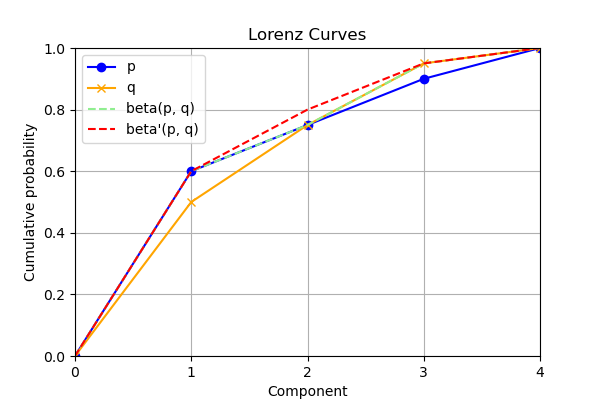
\includegraphics[scale=0.48]{images/join_first_attempt.png}
        \caption{Lorenz curves for the vector $p = (0.6, 0.15, 0.15, 0.1)$ and the vector $q = (0.5, 0.25, 0.20, 0.05)$, along with the join prototypes $\beta(p, q)$ and $\beta'(p, q)$.}
        \label{fig:first_join_attempt}
    \end{minipage}
    \hfill
    \begin{minipage}{0.48\textwidth} 
        \centering
        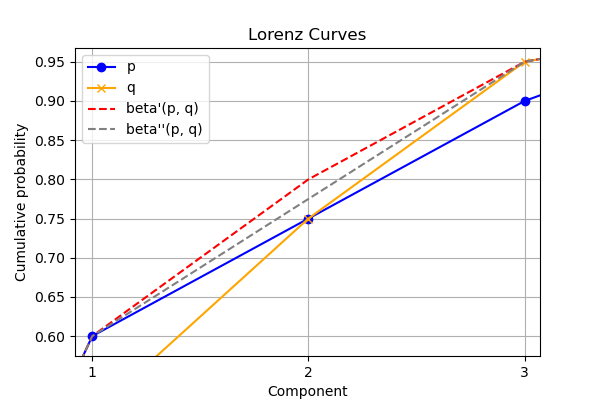
\includegraphics[scale=0.48]{images/join_second_attempt.png}
        \caption{Zoom on the region that visually shows that the $\beta'(p, q)$ vector is not the join, as there exist vectors such as $\beta''(p, q)$ that are majorized by it but still majorize both $p$ and $q$.} 
        \label{fig:second_join_attempt}
    \end{minipage}
\end{figure}

\noindent We have the following statement:

\begin{equation}
    p, q \prec (0.6, 0.175, 0.175, 0.05) \prec \beta'(p, q).
\end{equation}

The following definition provides the smoothing algorithm to apply to $\beta(p, q)$ to obtain the join of $p$ and $q$.

\begin{definition}[Concave dent smoothing algorithm] \label{def:smoothing_algorithm}
    Let $b = (b_1, ..., b_d)$, and let $j$ be the smallest integer in $\{2,...,d\}$ such that $b_j > b_{j-1}$. Moreover, let $i$ be the greatest integer in $\{1, 2, ..., j-1\}$ such that
    \begin{equation}
        b_{i-1} \geq \frac{\sum_{r=1}^{j}b_r}{j-i+1} \eqqcolon a.
    \end{equation}
    Let the probability distribution $c = (c_1, ..., c_d)$ be defined as
    \begin{equation}
        c_r = \begin{system}
                a, \quad \text{for} \; r = i, i+1, ..., j \\ % bon mon workaround pour avoir du displaystyle dans system nique \text lol
                b_r \quad \text{otherwise}.
              \end{system}
    \end{equation}
    This vector is the same as the original vector, but where the \textit{first} concave dent found in the Lorenz curve has been smoothed out.
\end{definition}

\begin{lemma}[Cicalese and Vaccaro, 2002 \cite{cicalese_supermodularity_2002}] \label{lem:join}
    For any $p, q \in \mathcal{P}^d$ we obtain $p \vee q$ in at most $d-1$ iterations\footnote{Smoothing a concave dent can lead to a concave dent with the following point, so there is at most $d-1$ concave dents to smoothe.} of the algorithm described in definition \ref{def:smoothing_algorithm} applied to the vector $\beta(p, q)$.
\end{lemma}

Lemmas \ref{lem:meet} and \ref{lem:join} conclude the proof sketch for the set $\mathcal{P}^d$ endowed with the majorization relation being a lattice, as we have found the lub and glb of any two vectors in $\mathcal{P}^d$. Working implementations of the join and meet algorithms in Python are available on the \href{https://github.com/traaldbjerg/MajoLat}{GitHub for the project}, which consists of a small library for majorization-related tasks such as plotting Lorenz curves or applying bistochastic matrices on probability vectors. The library can be used with QuTip which is a Python quantum information library for generating quantum state representations.


 
\subsection{Algebraic properties of the meet and join}

This section is based on Ref. \cite[pp. 39--41]{davey_introduction_2002}. In any lattice, the meet and the join can also be seen as two operations\footnote{This yields an equivalent definition of a lattice, which can be defined as a triple $\langle \mathcal{L}, \wedge, \vee \rangle$ with operations $\wedge, \vee$ acting on elements of $\mathcal{L}$. If they satisfy the properties listed above, an ordering $\sqsubseteq$ can then be derived from the triple by defining $a \sqsubseteq b \iff a \wedge b = a$.}
acting on elements of a set $\mathcal{L}$, which enjoy some useful properties.

\begin{itemize} \label{it:meet_join_properties}
    \item Commutativity: $a \wedge b = b \wedge a, \; a \vee b = b \vee a \quad \forall a, b \in \mathcal{L}$.
    \item Associativity: $a \wedge (b \wedge c) = (a \wedge b) \wedge c, \;
                            a \vee (b \vee c) = (a \vee b) \vee c \quad \forall a, b, c \in \mathcal{L}$.
    \item Idempotency: $a \wedge a = a, \; a \vee a = a \quad \forall a \in \mathcal{L}$.
    \item Absorption: $a \wedge (a \vee b) = a, \; a \vee (a \wedge b) = a \quad \forall a, b \in \mathcal{L}$.
\end{itemize}

While it is fairly clear how the algorithms from sections \ref{sec:meet} and \ref{sec:join} lead to commutativity, associativity, and idempotency, it might not be as clear why they lead to the absorption rule. Recall definition \ref{def:lattice} and the interpretation of glb and lub of the meet and join respectively. Then it becomes clearer that the first absorption rule for the majorization lattice states that \textit{the most ordered vector that is majorized by both $a$ and some vector that majorizes $a$ (and $b$) is none other than $a$}. Similarly, the second absorption rules states that \textit{the least ordered vector that majorizes both $a$ and some vector that is majorized by $a$ (and $b$) is $a$}. Yet another way to understand it is that this boils down to Corollary \ref{cor:comp_meet_join}: $a$ is necessarily comparable to $a \vee b$ (resp. $a \wedge b$) since by definition $a \prec a \vee b$ (resp. $a \succ a \wedge b$), and when two vectors are comparable their meet (resp. join) is simply the least ordered (resp. most ordered) of the two vectors, being $a$ in this case.

% parler du fait que les proprietes sont logiques dans la vision geometrique aussi ?

These properties are extremely helpful when working on proofs on the lattice, and will appear often in chapters \ref{chap:incomparability} and \ref{chap:volume}.



\section{Properties of the Shannon entropy on the lattice}

This section is based on Refs. \cite{cicalese_supermodularity_2002} and \cite{cicalese_information_2013}. The Schur-concavity of the Shannon entropy, which preserves the ordering of the majorization relation, has already been discussed in section \ref{sec:schur_shannon}. However, the Shannon entropy enjoys additional properties on the majorization lattice: \textit{supermodularity} and \textit{subadditivity}.



\subsection{Supermodularity} \label{sec:supermodularity}

\begin{definition} \label{def:supermodularity}
    A real-valued function $f$ defined on a lattice $\langle \mathcal{L}, \sqsubseteq, \wedge, \vee \rangle$ is \textit{supermodular} iff for any $a, b \in \mathcal{L}$
    \begin{equation}
        f(a \wedge b) + f(a \vee b) \geq f(a) + f(b).
    \end{equation}
\end{definition}


\begin{theorem}[Supermodularity of Shannon entropy] \label{th:shannon_supermodularity}
    The entropy function $H$ is supermodular on the majorization lattice, and so for all $p, q \in \mathcal{P}^d$,
    \begin{equation} \label{eq:supermodularity_shannon}
        H(p \wedge q) + H(p \vee q) \geq H(p) + H(q).
    \end{equation}
    Note that if $p \sim q$, there is trivially equality.
\end{theorem}

This property is quite useful when working on the lattice. The original proof is long and hinges on unintuitive index tricks, however one of the first results of this master thesis is to prove a generalization of theorem \ref{th:shannon_supermodularity} which is applicable to a broader class of functions than only Shannon entropy, however it only works in specific cases. As such we will leave the proof for section \ref{sec:alternative_supermodularity}. We will also encounter the reverse concept of \textit{submodularity} later on.

\begin{definition} \label{def:submodularity}
    A function $f$ defined on a lattice $\langle \mathcal{L}, \sqsubseteq, \wedge, \vee \rangle$ is \textit{submodular} iff for any $a, b \in \mathcal{L}$, $-f$ is supermodular. Alternatively,
    \begin{equation}
        f(a \wedge b) + f(a \vee b) \leq f(a) + f(b).
    \end{equation}
\end{definition}



\subsection{Subadditivity} \label{sec:subadditivity}

\begin{definition}[Subadditivity] \label{def:subadditivity}
    A real-valued function $f$ defined on a lattice $\langle \mathcal{L}, \sqsubseteq, \wedge, \vee \rangle$ is \textit{subadditive} iff for any $a, b \in \mathcal{L}$
    \begin{equation}
        f(a \wedge b) \leq f(a) + f(b).
    \end{equation}
\end{definition}

\begin{theorem}[Subadditivity of the Shannon entropy] \label{th:shannon_subadditivity}
    The entropy function $H$ is subadditive on the majorization lattice, so for all $p, q \in \mathcal{P}^d$
    \begin{equation}
        H(p \wedge q) \leq H(p) + H(q).
    \end{equation}
\end{theorem}

One of the first results of this master thesis is to prove a stronger version of theorem \ref{th:shannon_subadditivity} which is applicable to a broader class of functions than only Shannon entropy. Moreover, this time our proof has no additional condition, and so theorem \ref{th:shannon_subadditivity} becomes a corollary of our theorem. We will leave the proof for section \ref{sec:alternative_subadditivity}. We will also encounter the reverse concept of \textit{superadditivity} later on.

\begin{definition}[Superadditivity] \label{def:superadditivity}
    A real-valued function $f$ defined on a lattice $\langle \mathcal{L}, \sqsubseteq, \wedge, \vee \rangle$ is \textit{superadditive} iff for any $a, b \in \mathcal{L}$, $-f$ is subadditive. Alternatively,
    \begin{equation}
        f(a \wedge b) \geq f(a) + f(b).
    \end{equation}
\end{definition}



\subsection{Entropic distance on the lattice} \label{sec:entropic_distances}

Shannon entropy can be used to define an entropic distance on the lattice, which allows us to quantify how far away two probability vectors are from each other on the lattice. We will use it quite a lot in chapter \ref{chap:incomparability} to quantify the amount of incomparability between 2 probability vectors.

\begin{definition}[Entropic distance] \label{def:entropic_distance}
    For all $p, q \in \mathcal{P}^d$, we define
    \begin{equation}
        d(p, q) = H(p) + H(q) - 2H(p \vee q).
    \end{equation}
\end{definition}

\begin{theorem}[Cicalese, Gargano and Vaccaro, 2013]
    $d$ is a distance on $\mathcal{P}^d$, meaning that it satisfies the following properties:
    \begin{itemize}
        \item Symmetry: $d(p, q) = d(q, p)$,
        \item Positivity: $d(p, q) \geq 0$ \text{with equality} iff $p = q$,
        \item Triangular inequality: $d(p, q) \leq d(p, t) + d(t, q)$.
    \end{itemize}
\end{theorem}

This distance has a few non-intuitive properties, but remains a rigorous notion of distance nonetheless. % expliquer geometrie hyperbolique et faire un diagramme ?
We will also use a quasidistance going through the meet instead of the join.

\begin{definition}[Meet-based entropic quasidistance] \label{def:entropic_quasidistance}
    For all $p, q \in \mathcal{P}^d$, we define
    \begin{equation}
        d(p, q) = 2H(p \wedge q) - H(p) - H(q).
    \end{equation}
\end{definition}

This notion of distance is unfortunately not as foolproof as the first one, which goes through the join. In particular, while it does satisfy symmetry and positivity, it fails the triangular inequality in some cases. For example, consider vectors TROUVER EXEMPLE. As such, one can not use it as a rigorous notion of distance, but it still has a few applications nonetheless.

\begin{figure}[h!]
    \centering
    \begin{tikzpicture}[scale=0.9]
        % draw cone of p
        \coordinate (A) at (-2, 1);
        \coordinate (B) at (2, -1);
        \coordinate (C) at (-1, 4);
        \coordinate (D) at (1, -4);
        \draw [name path=A--C] (A) -- (C) node[midway, above, sloped] {$d(p, p \wedge q)$};
        \draw [name path=C--B] (C) -- (B) node[midway, above, sloped] {$d(q, p \wedge q)$};
        \draw [name path=B--D] (B) -- (D) node[midway, below, sloped] {$d(q, p \vee q)$};
        \draw [name path=D--A] (D) -- (A) node[midway, below, sloped] {$d(p, p \vee q)$};
        %\path [name intersections={of=A--B and C--D,by=E}];
        \node [fill=black,inner sep=1pt,label=0:$p$] at (A) {};
        \node [fill=black,inner sep=1pt,label=0:$q$] at (B) {};
        \node [fill=black,inner sep=1pt,label=0:$p \wedge q$] at (C) {};
        \node [fill=black,inner sep=1pt,label=0:$p \vee q$] at (D) {};
        % draw cone of q
        \coordinate (F) at (-0.666,3);
        \coordinate (G) at (3.333, -3);
        %\draw [name path=F--G] (F) -- (G);
        \coordinate (H) at (0.666,-3);
        \coordinate (I) at (4.666,3);
    \end{tikzpicture}
    \caption{Depiction of the incomparability diamond $p, q, p \wedge q, p \vee q$ generated by two incomparable vectors $p, q \in \mathcal{P}^d$. Supermodularity implies that $d(p, p\vee q) = H(p) - H(p \vee q) \leq d(q, q \wedge p) = H(p \wedge q) - H(q)$, which seems to indicate some form of hyperbolic metric on the lattice where segments higher up are larger despite the parallel lines.} 
    \label{fig:hyperbolic_geometry}
\end{figure}

An interpretation of these notions of distance is given in figure \ref{fig:hyperbolic_geometry}. Notably, the distance $d$ seems to induce some form of hyperbolic metric in the majorization lattice, in the sense that two segments that look identical in our geometrical representation (due to parallel lines) are not according to this notion of distance. For example, in any incomparable diamond $p, q, p \wedge q, p \vee q$ we have $d(p, p\vee q) = H(p) - H(p \vee q) \leq d(q, q \wedge p) = H(p \wedge q) - H(q)$ by supermodularity, even though when looking at the representation one would get the idea that the 2 distances are equal. In general, segments become larger the higher they are on the lattice. This intuition is helpful to understand some results of chapter \ref{chap:incomparability}. Finally, the following lemma will help us see another unusual property of this entropic distance, represented on figure \ref{fig:triangular_lemma}.

\begin{lemma} (Cicalese, Gargano and Vaccaro, 2013 \cite{cicalese_information_2013}) \label{lem:comp_future} 
    The join $p \vee q$ of two probability vectors $p, q \in \mathcal{P}^d$ saturates the triangular inequality for the entropic distance $d(p, q) = H(p) + H(q) - 2H(p \vee q)$.
\end{lemma}

\begin{proof}
    Let $p, q \in \mathcal{P}^d$. We have
    \begin{align}
        d(p, p \vee q) + d(p \vee q, q) &= H(p) + H(p \vee q) - 2H(p \vee (p \vee q)) + H(p \vee q) \nonumber \\
        &\quad \quad + H(q) - 2H((p \vee q) \vee q) \\
        &= H(p) + H(p \vee q) - 2H(p \vee q) + H(p \vee q) + H(q) \nonumber\\
        &\quad \quad - 2H(p \vee q) \\
        &= H(p) + H(q) - 2H(p \vee q) \\
        &= d(p, q),
    \end{align}
    where we have used associativity of successive joins to simplify the expressions. \qedhere
\end{proof}

\begin{figure}[h!]
    \centering
    \begin{tikzpicture}[scale=0.9]
        % draw cone of p
        \coordinate (A) at (-1, 1.5);
        \coordinate (B) at (2, -3);
        \draw[dotted] [name path=A--B, color=gray] (A) -- (B);
        \coordinate (C) at (-2,-3);
        \coordinate (D) at (1,1.5);
        \draw[dotted] [name path=C--D, color=gray] (C) -- (D);
        \path [name intersections={of=A--B and C--D,by=E}];
        \node [fill=black,inner sep=1pt,label=90:$p$] at (E) {};
        % draw cone of q
        \coordinate (F) at (0.944,1.5);
        \coordinate (G) at (3.833, -3);
        \draw[dotted] [name path=F--G, color=gray] (F) -- (G);
        \coordinate (H) at (1.166,-3);
        \coordinate (I) at (3.966,1.5);
        \draw[dotted] [name path=H--I, color=gray] (H) -- (I);
        \path [name intersections={of=F--G and H--I,by=J}];
        \node [fill=black,inner sep=1pt,label=45:$q$] at (J) {};
        %intersections of the 2 cones
        %\path [name intersections={of=F--G and C--D,by=K}];
        \path [name intersections={of=H--I and A--B,by=L}];
        %\node [fill=black,inner sep=2pt,label=0:$p \wedge q$] at (K) {};
        \node [fill=black,inner sep=1pt] at (L) {};
        \node [inner sep=4pt, label=270:$p \vee q$] at (L) {}; % virtual point to set the label further away (otherwise the fill gets bigger too)
        % draw the 3 distances
        \draw [name path=E--J] (E) -- (J) node[midway, above, sloped] {$d(p, q)$};
        \draw [name path=E--L] (E) -- (L) node[midway, below, sloped] {$d(p, p \vee q)$};
        \draw [name path=L--J] (L) -- (J) node[midway, below, sloped] {$d(q, p \vee q)$};

    \end{tikzpicture}
    \caption{Depiction of the saturated triangular inequality $d(p, q) = d(p, p \vee q) + d(p \vee q, q)$ from Lemma \ref{lem:comp_future} for two incomparable vectors $p, q \in \mathcal{P}^d$.}
    \label{fig:triangular_lemma}
\end{figure}

A way to interpret this result is that the distance always \textit{goes through the join} when two vectors are incomparable, instead of measuring the "segment joining the two vectors" directly.